\documentclass[main.tex]{subfiles}
\begin{document}

\section{Постановка задачи}
Поставлена задача линейного программирования:
\begin{equation}\label{eq:initial}
\left\{
\begin{array}{ll} 
x_1-2x_2+2x_3 \le 6\\
x_1+2x_2+x_3+x_4=24\\
2x_1+x_2-4x_3+1=30\\
-x_1+4x_2+2x_4 \ge -6\\
x_i \ge 0 \hspace{3pt} \forall i \in \{1;3\}
\end{array}
\right.
\end{equation}
$$ 8x_1 + 3x_2 + 4x_3 + 2x_4 \longrightarrow min $$
\begin{enumerate}
\item Привести задачу к виду, необходимому для применения симплекс-метода.
\item Построить к данной задаче двойственную и также привести к виду, необходимому для применения симплекс-метода.
\item Решить обе задачи симплекс-методом с выбором начального приближения методом искусственного базиса.
\item Решить обе задачи методом перебора крайних точек.
\item Разработать схему восстановления прямой задачи по решению двойственной.
\end{enumerate}
Алгоритмы, требуемые для решения задачи, реализовать в таком виде, чтобы их можно было использовать в качестве подпрограмм в следующих лабораторных работах.
\section{Исследование применимости метода}
Алгоритм симплекс-метода, приведённый в пособии \cite{petuh} и описанный ниже, применим к задачам линейного программирования на нахождение минимума. Метод работает с задачами в канонической форме при всяких вещественных значениях компонент $A \in \mathds{R}_{m\times n}, b \in \mathds{R}_m, c \in R_n$ с условием: матрица $A$ имеет ранг $m$ (следовательно, существует хотя бы один опорный вектор).\\
После приведения задачи (\ref{eq:initial}) (или двойственной к ней) к каноническому виду получается система с матрицей $ 9 \times 4 $ ранга $4$, следовательно, условие выполнено.\\

\newpage
\section{Описание алгоритмов}
\subsection{Алгоритм перевода из общей в каноническую форму}
\textbf{Вход}: система
% TODO написать вид системы
\begin{enumerate}
\item Проверяем знаки в системе
\item Если <<$\le$>>, то к левой части добавляем $w[i]$, если <<$\ge$>>, то из левой части вычитаем $w[i]$, $w[i]\ge0$.
\item Знаки неравенства в системе заменяем на равенство.
\item Производим замену переменных: если $x[i]\le0$, то $x'[i]=-x[i]\ge0$; если $x[i]$ любого знака, то $x[i]=u[i]-v[i]$, $v[i],u[i] \ge 0$.
\end{enumerate}
\subsection{Алгоритм построения двойственной задачи}
Для простоты алгоритма будем рассматривать задачу максимума:
\begin{equation}\label{eq:maxproblem}
\begin{array}{ll}
(x[N],c[N])\longrightarrow \max_{x[N]}, x[N] \in S, x[N] \ge 0\\
S :=\{x[N]|A[M,N]\cdot x[N] \gtreqless b[M]\}, x[N] \ge 0
\end{array}
\end{equation}
Если перед нами стоит задача минимума, то домножим вектор коэффициентов матрицы цели на $-1$.
\begin{enumerate}
\item Транспонируем заданную матрицу $А$
\item Новый вектор коэффицентов, стоящий в системе справа, равен вектору коэффициентов функции цели (\ref{eq:maxproblem}).
\item Новый вектор коэффициентов функции цели равен вектору коэффицентов, стоящему в системе (\ref{eq:maxproblem}) справа.
\item Если ограничение на $x[i]\ge0$, то $i$-ая строка новой системы имеет знак "$\ge$".
Если нет ограничения на знак, то $i$-ая строка новой системы имеет знак <<$=$>>.
\item Если ограничение $i$-ой строки в исходной системе <<$\le$>> (тк рассматриваем задачу  максимума), то ограничение на знак новой переменной $y[i]\ge0$.
Если ограничение $i$-ой строки в исходной системе "$=$", то $y[i]$ любого знака.
\item Если исходная задача на поиск максимума, то двойственная на поиск минимума.
\end{enumerate}
\subsection{Алгоритм симплекс-метода и связанные процедуры}
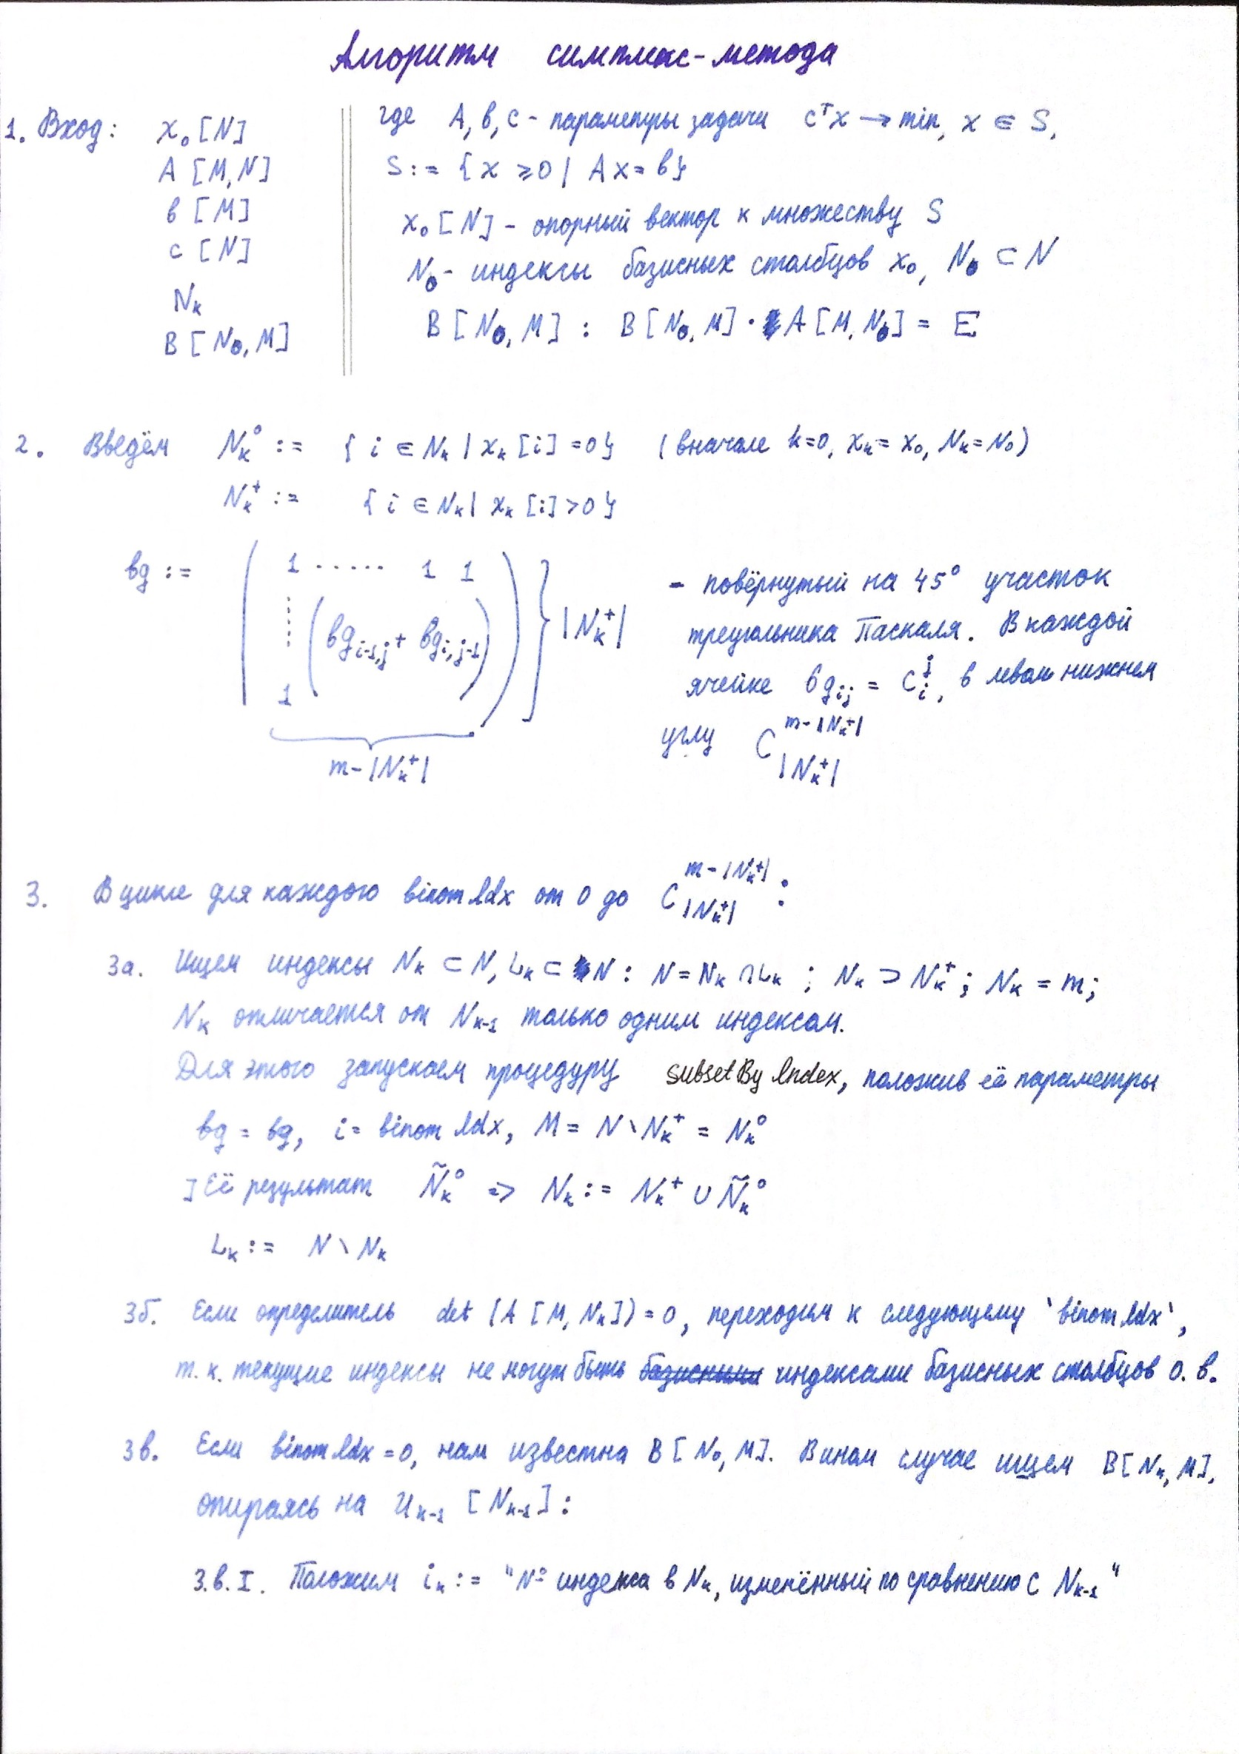
\includepdf[pages=-]{simplexEtcWritten.pdf}
\subsection{Алгоритм перебора опорных векторов}
Опорные векторы можно искать прямо по определению, перебирая все возможные базисы и находя соответствующие ненулевые коэффициенты из решения СЛАУ. Множества входящих в базис столбцов будем определять с помощью метода \textit{subsetByIndex}, описанной в предыдущем разделе. Также будем пользоваться процедурой \textit{inv}, описываемой в следующем разделе, для нахождения обратной матрицы при решении СЛАУ.\\

\SetKwRepeat{Do}{do}{while}
\begin{algorithm}[H]
	\KwData{$A[M,N], b[M], c[N]$ -- параметры задачи линейного программирования, поставленной в канонической форме\; $m=|M|, n=|N|$}
	\KwResult{опорный вектор $x_*[N]$, минимизирующий целевую функцию $(x[N],c[N])$}
	инициализация матрицы $bg[N,M]$ биномиальных коэффициентов\;
	$V:=\emptyset$ -- будущий список опорных векторов\;
	\For{$i$ в диапазоне $\{0;C_m^n\}$}{
		$N_k := $  subsetByIndex($i$,$bg$)\;
		\If{$det(A[M,N_k])\ne 0$}{
			$x[N_k]:=$ inv($A[M,N_k], b[M]$)\;
			Дополняем нулями до $x[N]$\;
			Добавляем $x[N]$ в $V$\;
		}
	}
	Выбираем $x_*$  -- любой вектор из $V$\;
	\For{$v \in V$}{
		\If{$(v,c) < (x_*,c)$}{
			$x_*:=v$\;
		}
	}
	
	\caption{Метод перебора опорных векторов решения задачи линейного программирования в канонической форме}
\end{algorithm}

\subsection {Алгоритм нахождения обратной матрицы}
\section{Результаты решения задачи}
\section{Оценка достоверности полученного результата}
\begin{thebibliography}{99}
	\bibitem{petuh} Петухов Л. В. Методы оптимизации. Задачи выпуклого программирования: учеб. пособие / Л. В. Петухов, Г. А. Серёгин, Е. А. Родионова. -- СПб.: Изд-во Политехн. ун-та, 2014. -- 99 с.
\end{thebibliography}

\end{document}